\documentclass[11pt]{article}

\usepackage[utf8]{inputenc}
\usepackage[T1]{fontenc}
\usepackage[margin=1in]{geometry}
\usepackage{graphicx}
\usepackage{booktabs}
\usepackage{xcolor}
\usepackage{listings}
\usepackage{amsmath}
\usepackage{enumitem}
\usepackage{caption}
\usepackage[colorlinks=true,linkcolor=blue,urlcolor=blue,citecolor=blue]{hyperref}

% Style for the terminal / code listings
\definecolor{shellbg}{gray}{0.95}
\lstdefinestyle{shell}{
  basicstyle=\ttfamily\small,
  breaklines=true,
  breakatwhitespace=true,
  breakindent=0pt,
  postbreak=\mbox{\textcolor{gray}{$\hookrightarrow$}\space},
  frame=single,
  framesep=6pt,
  rulecolor=\color{gray!40},
  backgroundcolor=\color{shellbg},
  keepspaces=true,
  columns=fullflexible,
  showstringspaces=false,
  xleftmargin=4pt,
  xrightmargin=4pt,
}

\title{\textbf{Beamline Voltage Optimization}\\[2pt]
       \large A Hands-On Activity with SIMION and Optuna}
\author{MIT--Medell\'in Hackathon}
\date{}

\setlength{\emergencystretch}{3em}

\begin{document}
\maketitle

% ===========================================================================
\section{The goal}
% ===========================================================================

You are given a small \emph{ion beamline} simulated in SIMION. A beam of ions
is launched at one end, and your job is to steer and focus it so that as many
ions as possible reach a detector at the other end. How well the beamline does
this is called its \textbf{transmission}:
\[
  \text{Transmission} \;=\;
  \frac{\text{ions that reach the detector}}{\text{ions launched } (500)}
  \;\times\; 100\,\%.
\]

The catch: the transmission depends on the \emph{voltages} we put on the
electrodes, and there are many electrodes. Trying combinations by hand is
hopeless. Instead, you will let an optimization library called \textbf{Optuna}
search for the best voltages automatically, using SIMION as the ``referee''
that scores every guess. \textbf{Your final answer is the set of voltages that
maximizes transmission.}

\begin{figure}[h]
  \centering
  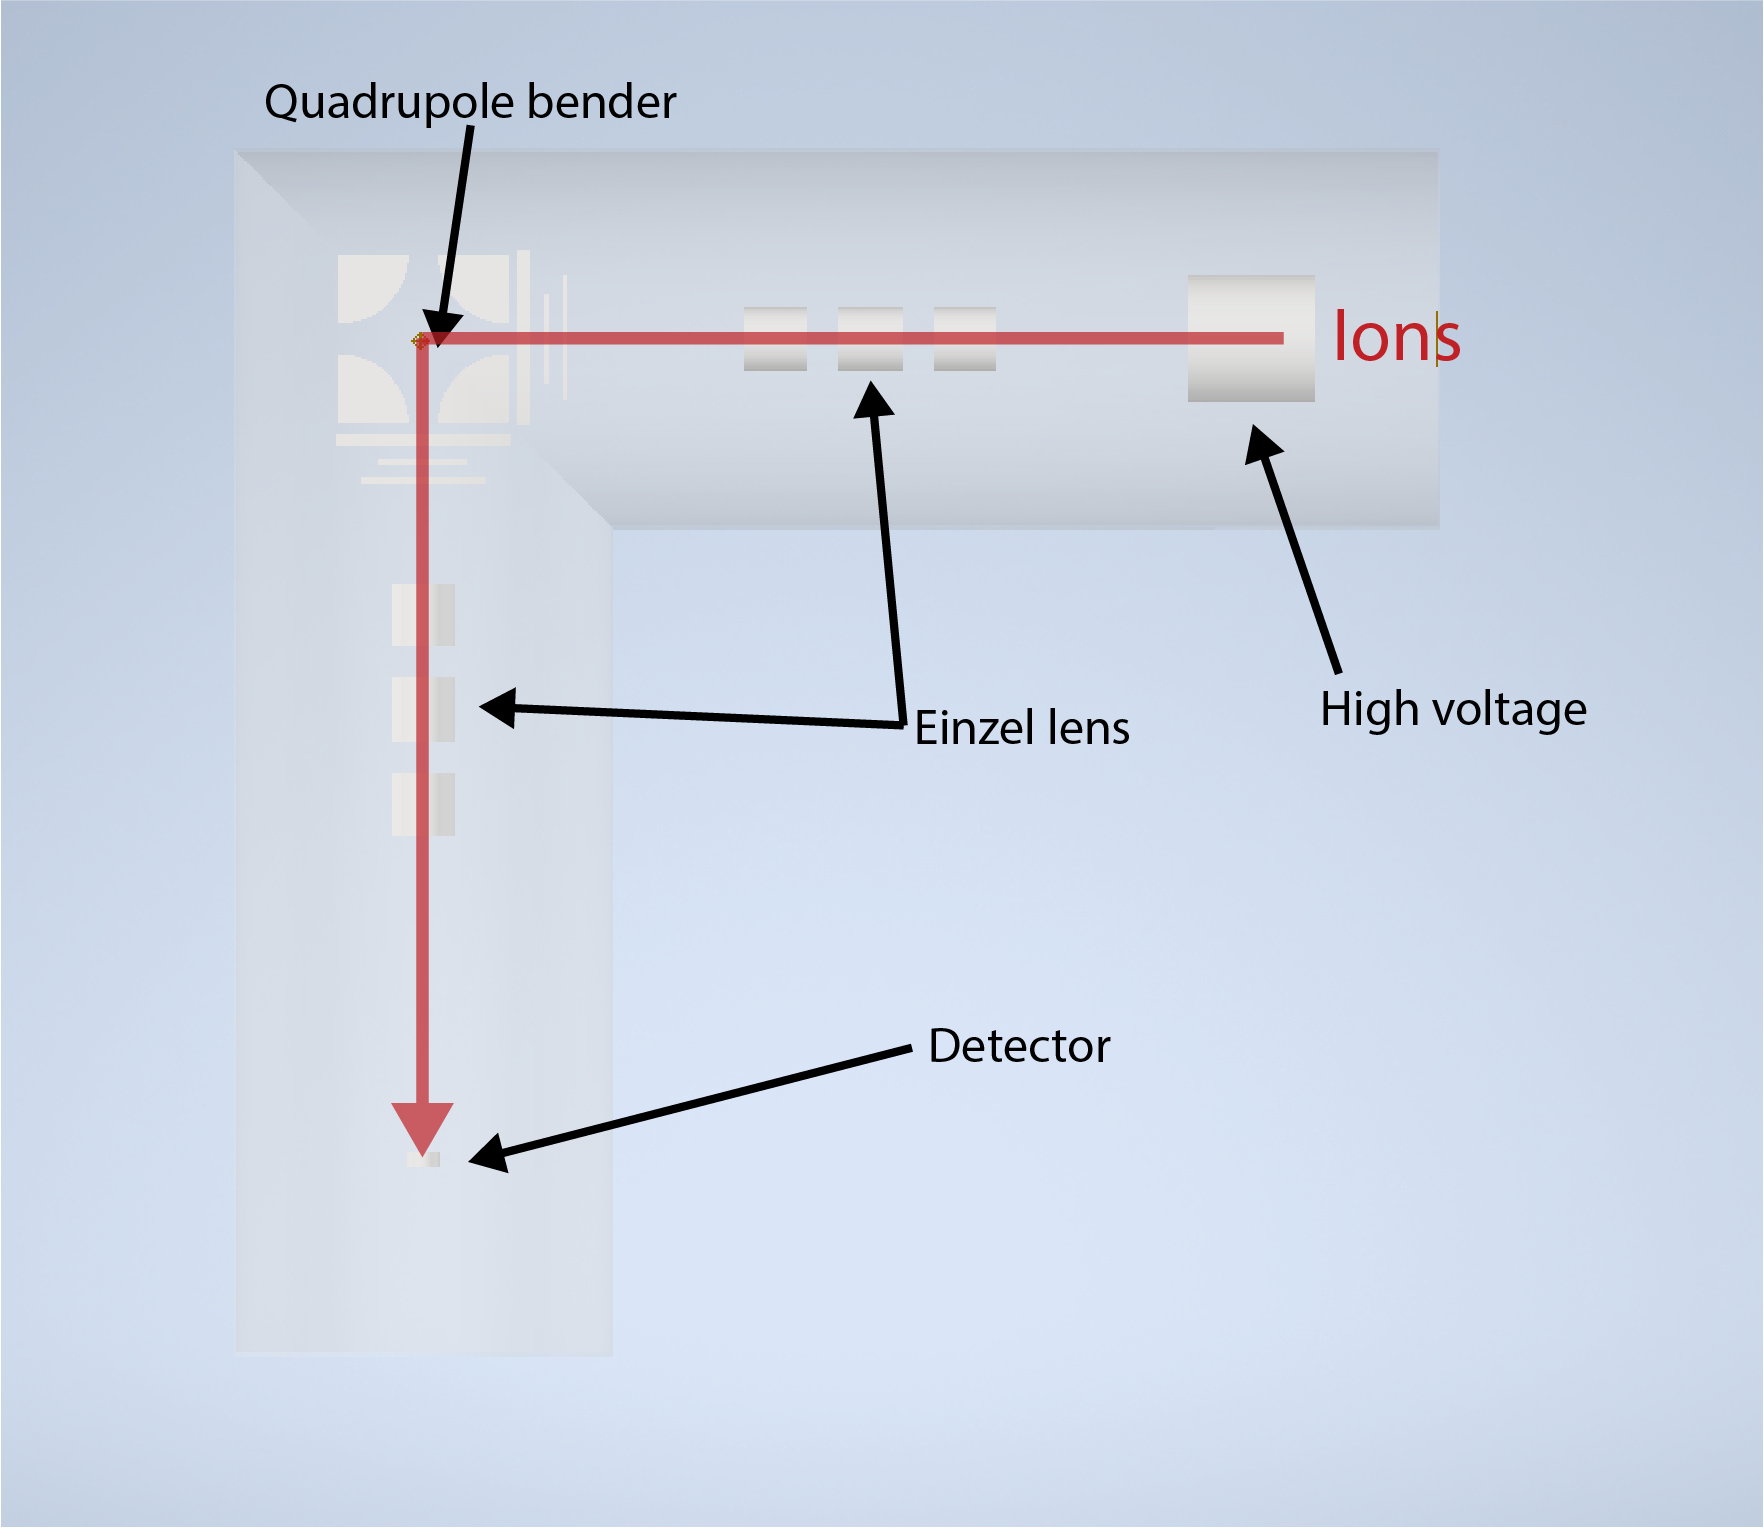
\includegraphics[width=0.62\textwidth]{ExperimentalSetup.png}
  \caption{The beamline. Ions are born inside the \emph{high-voltage} cage on
  the right and travel left through two \emph{Einzel lenses} (which focus the
  beam). The \emph{quadrupole bender} turns the beam $90^\circ$ at the corner,
  and the ions then travel down to the \emph{detector}. In simulation
  coordinates the beam starts at $(395, 75, 77)$\,mm moving along $-x$, is bent
  into $+z$, and is collected in a small box around $(76, 76, 405)$\,mm.}
  \label{fig:setup}
\end{figure}

% ===========================================================================
\section{The simulation files}
% ===========================================================================

All of these files live together in one \emph{project folder}, the same folder
you keep \texttt{optimizer.py} in. The optimizer finds that folder
automatically and uses \emph{relative} paths, so it does not matter where the
folder sits on your particular computer (the drive letter and the path will be
different on every machine). Here is what each kind of file is for.

\subsection{STL files: the geometry}
The \texttt{electrode\_1.stl}, \texttt{electrode\_2.stl}, \dots files are 3D
models (exported from CAD) of the \emph{shape} of each metal electrode: the
high-voltage cage, the pipe, the lens rings, the bender, the plates, and the
detector. They describe \emph{where the metal is}, but not what voltage it is
at. SIMION reads these shapes to build the simulation.

\subsection{The \texttt{.PA\#} and \texttt{.PA0} files: the electric fields}
A \emph{potential array} (PA) is SIMION's grid describing the electric setup in
space. There are three kinds, and only the first one is given to you:
\begin{itemize}[nosep]
  \item \texttt{electrode\_.PA\#}: the \emph{definition} file. It records the
        geometry (which grid points are metal, and which electrode number
        each belongs to) but \textbf{not} the electric field yet. This is the
        single file you start from. \emph{You generate the other two from it} by
        ``refining'' (see Step~0 in Section~\ref{sec:terminal}).
  \item \texttt{electrode\_.PA1}, \texttt{electrode\_.PA2}, \dots,
        \texttt{electrode\_.PA19}: one \emph{solved} field per electrode,
        computed with that electrode at unit voltage and all others grounded.
        Solving these is the slow step, but it only has to be done once.
  \item \texttt{electrode\_.PA0}: the combined ``\emph{fast-adjust}'' array.
        Because fields add up linearly, SIMION can take your chosen voltage for
        every electrode and \emph{instantly} build the total field by scaling
        and summing the per-electrode arrays, with no slow re-solving. This is
        what lets the optimizer test thousands of voltage combinations quickly.
\end{itemize}
The \texttt{.PA1\dots PA19} and \texttt{.PA0} files are large (hundreds of MB
each), which is why they are \emph{not} shipped to you; you create them once
on your own machine by refining the small \texttt{.PA\#}.

\subsection{The \texttt{.fly2} file: the ion beam}
\texttt{SimpleSetUp.fly2} defines the particles we shoot in: \textbf{500}
singly-charged silicon ions ($^{28}$Si$^+$, mass 28\,amu, charge $+1$), with a
kinetic energy of about 15\,eV, launched from position $(395, 75, 77)$\,mm in a
$15^\circ$ cone aimed along the $-x$ direction. Every run flies this same beam,
so any change in transmission is due to the \emph{voltages}, not the beam.

\subsection{The \texttt{.iob} file: the workbench}
\texttt{SimpleSetUp.iob} is the SIMION ``workbench'': it ties everything
together (the geometry, the potential arrays, the beam, and the recording
settings) into one runnable simulation. When we tell SIMION to ``fly'', this
is the file we point it at.

% ===========================================================================
\section{Which voltages are fixed, and which you optimize}
% ===========================================================================

Not every electrode is a free knob. Some \emph{must} stay at a set voltage
because of the role they play (file \texttt{ElectrodesMaps.txt}):

\begin{itemize}[nosep]
  \item \textbf{High-voltage cage ($+500$\,V).} This is the charged enclosure
        where the ions are created. Its potential sets the starting energy of
        the beam, so it is a fixed property of the source, not a tuning knob.
  \item \textbf{Grounding pipe and ground plates ($0$\,V).} These are the
        reference (``earth'') electrodes and electrostatic shields. Ground
        \emph{is} the zero of our voltage scale; changing it would not steer
        the beam, it would just move the reference.
  \item \textbf{Detector ($-2000$\,V).} The detector is held strongly negative
        so it attracts and collects the positive ions. It is the measuring
        device at the end of the line, so its voltage is fixed too.
\end{itemize}

Everything that \emph{shapes} the beam (the lenses, the bender, and the
steering plates) is left free. \textbf{Those are the voltages you optimize.}
In \texttt{ElectrodesMaps.txt} they are exactly the electrodes that have
\emph{no} value written next to them. There are eight of them, so this is an
8-dimensional search.

\begin{table}[h]
\centering
\caption{The electrodes of the beamline.}
\begin{tabular}{clc}
\toprule
\textbf{Electrode(s)} & \textbf{Component} & \textbf{Voltage} \\
\midrule
1        & High-voltage cage (ion source)        & $+500$\,V (fixed) \\
2        & Grounding pipe                        & $0$\,V (fixed) \\
\textbf{3}   & Einzel lens 1 (biased element)  & \textbf{optimize} \\
4, 5     & Einzel lens 1 (grounded elements)   & $0$\,V (fixed) \\
\textbf{6}   & Einzel lens 2 (biased element)  & \textbf{optimize} \\
7, 8     & Einzel lens 2 (grounded elements)   & $0$\,V (fixed) \\
\textbf{9--12} & Quadrupole bender (four parts)  & \textbf{optimize} \\
13, 14   & Ground plates                         & $0$\,V (fixed) \\
\textbf{15}  & Voltage / steering plate 1        & \textbf{optimize} \\
16, 17   & Ground plates                         & $0$\,V (fixed) \\
\textbf{18}  & Voltage / steering plate 2        & \textbf{optimize} \\
19       & Detector                              & $-2000$\,V (fixed) \\
\bottomrule
\end{tabular}
\end{table}

So the optimizer is free to choose voltages for electrodes
\textbf{3, 6, 9, 10, 11, 12, 15, and 18}; all the others are pinned to the
values above on every single run.

\paragraph{Keep the voltages physical.} For each free electrode you must give
the optimizer a \emph{range} of voltages to search within. Choose those ranges
to match what real lab power supplies can actually produce; they cannot
output millions of volts. As a rule of thumb, $\pm 500$\,V is comfortably
available, and \textbf{$\pm 1000$\,V is the maximum you should allow}. A voltage
the power supply cannot deliver is useless, even if the simulation ``likes''
it, so do not let the search wander beyond that. (The fixed $+500$\,V source and
$-2000$\,V detector run on their own dedicated high-voltage supplies, which is
why those two are allowed to sit outside the $\pm 1000$\,V range.)

% ===========================================================================
\section{Running SIMION from the terminal}
\label{sec:terminal}
% ===========================================================================

Once SIMION is set up, almost everything happens through a few command-line
instructions. You run \textbf{Step~0 once} at the very beginning; the optimizer
then runs \textbf{Steps~1 and 2 automatically} for every guess it makes (and you
can also run those two by hand to see what they do).

\paragraph{Make sure ``\texttt{simion}'' is runnable first.} Every command below
starts with the word \texttt{simion}. For your terminal to understand it, your
computer has to know where SIMION is installed, and that folder is different
on every machine. If you type \texttt{simion} and see an error like
``\texttt{simion is not recognized}'' (Windows) or ``\texttt{command not found}'',
pick one of these:
\begin{itemize}[nosep]
  \item \textbf{Add SIMION to your PATH.} Add the SIMION install folder (the one
        containing \texttt{simion.exe}, normally
        \texttt{C:\textbackslash\allowbreak Program Files\textbackslash\allowbreak SIMION-8.1}) to your
        system's \emph{Path} environment variable, then open a \emph{new}
        terminal. Now plain \texttt{simion} works everywhere, exactly as written
        below.
  \item \textbf{Or write the full path to the program} in every command, in
        place of the word \texttt{simion}. In PowerShell you put the \texttt{\&}
        call operator in front of the quoted path, for example:
\end{itemize}

\begin{lstlisting}[style=shell]
& "C:\Program Files\SIMION-8.1\simion.exe" --nogui refine "electrode_.PA#"
\end{lstlisting}

\noindent (The Python optimizer already knows where SIMION is from the
\texttt{SIMION\_INSTALL\_DIR} setting in its CONFIG, so this only matters for
commands \emph{you} type by hand.)

\paragraph{The SIMION manual.} The easiest reference is the PDF included with
this activity, \texttt{simion8manual.pdf}. It documents an older SIMION version,
but the command-line tools are the same, and they are all described in
\textbf{Appendix~M (Command Line Interface)}; look there for every option of
\texttt{refine}, \texttt{fastadj} and \texttt{fly}.

Your installed SIMION also ships the newer, complete manual as
\texttt{simion.chm} in the SIMION folder (the one that holds
\texttt{simion.exe}); search it for ``command line''. Note that \texttt{.chm} is
a Windows Help file, and Windows often \textbf{blocks} it (via Smart App
Control, or the file's ``Mark of the Web''), so it may open blank or say
``Navigation to the webpage was canceled''. To allow it: right-click
\texttt{simion.chm} $\to$ \emph{Properties} $\to$ tick \emph{Unblock} $\to$
\emph{OK}. If Smart App Control still blocks it, copy it to a local folder such
as your Desktop and open it from there.

\paragraph{Step 0: refine the potential array (\texttt{refine}), do this once.}
You are given only the geometry file \texttt{electrode\_.PA\#}. ``Refining'' is
the step where SIMION solves the electric field for the geometry and writes out
the heavy field files: \texttt{electrode\_.PA0} plus the per-electrode arrays
\texttt{electrode\_.PA1\dots PA19}. Run it once from the project folder:

\begin{lstlisting}[style=shell]
simion --nogui refine "electrode_.PA#"
\end{lstlisting}

\noindent This can take a few minutes and some memory; that is normal, because
you are solving a field on a grid of millions of points. You only ever do it
once; after that the field files exist and flying is fast. If you change the
\emph{geometry}, refine again; if you only change \emph{voltages}, you do not.

\paragraph{Step 1: set the voltages (\texttt{fastadj}).}
The \texttt{fastadj} sub-command writes a voltage onto every electrode of the
fast-adjust \texttt{.PA0} array. It takes the array file followed by a
comma-separated list of \texttt{electrode=voltage} pairs. \emph{Assembling this
command is your Task~1b in \texttt{optimizer.py}.}

\paragraph{Step 2: fly the ions and see where they land (\texttt{fly}).}
The \texttt{fly} sub-command sends the 500 ions through the field defined by the
workbench file and prints where each one lands. \emph{Assembling this command is
your Task~1a in \texttt{optimizer.py}.}

\noindent You build both commands yourself, from the pieces in the table below
and the SIMION manual (\texttt{simion8manual.pdf}, Appendix~M; see the note
above). Here is what each piece does:

\begin{table}[h]
\centering
\caption{What each part of the SIMION command means.}
\renewcommand{\arraystretch}{1.25}
\begin{tabular}{p{0.40\textwidth} p{0.54\textwidth}}
\toprule
\textbf{Part of the command} & \textbf{What it does} \\
\midrule
\texttt{simion} & Launches the SIMION program. \\
\texttt{-{}-nogui} & Runs it \emph{headless} (no graphical window) so a script
  can drive it automatically. \\
\texttt{fly} & The sub-command that actually simulates (``flies'') the ions
  through the field. \\
\texttt{fastadj} & The sub-command that instantly sets electrode voltages,
  using the fast-adjust \texttt{.PA0} array. \\
\texttt{"electrode\_.PA0"} & The potential-array file whose voltages we are
  setting. (Quoted because the folder path contains a space.) \\
\texttt{1=500,2=0,\dots} & The list of \texttt{electrode=voltage} assignments.
  We set \emph{every} electrode each time so each run is fully reproducible. \\
\texttt{-{}-recording-output=out.txt} & The file SIMION writes its recorded
  data to. \\
\texttt{-{}-retain-trajectories=0} & Do \emph{not} keep every ion's full flight
  path in memory, since we only need where each ion ends up. Faster and lighter. \\
\texttt{-{}-restore-potential=0} & Do \emph{not} undo the voltages after the
  run; leave the field we just set in place. \\
\texttt{-{}-programs=0} & Run the batch flight without extra user-program
  passes, keeping each run lean. \\
\texttt{"SimpleSetUp.iob"} & The workbench (geometry + beam + recording) we
  are flying. \\
\bottomrule
\end{tabular}
\end{table}

After the flight, SIMION prints one line of the form
\texttt{xyz(76, 75, 405)mm} for each ion that reaches the detector. The
optimizer counts those lines; that count is the transmission score.

% ===========================================================================
\section{What you are going to do}
% ===========================================================================

Make sure you have already done Step~0 (refined \texttt{electrode\_.PA\#}) so the
field files exist. Then you run a single Python program,
\texttt{optimizer.py}:

\begin{lstlisting}[style=shell]
python optimizer.py
\end{lstlisting}

\noindent Behind the scenes it repeats this loop (a method called
\emph{Bayesian optimization}):

\begin{enumerate}[nosep]
  \item \textbf{Optuna proposes} a voltage for each of the 8 free electrodes
        (within ranges you can edit at the top of the file).
  \item The script \textbf{sets} those voltages with \texttt{fastadj}.
  \item SIMION \textbf{flies} the 500 ions with \texttt{fly}.
  \item The script \textbf{counts} how many ions reached the detector; that
        count is the score.
  \item Optuna \textbf{learns} from the score and proposes a smarter set of
        voltages next time.
\end{enumerate}

After all the trials, the best-scoring set of voltages is your result. Results
are also saved to \texttt{beamline\_results.csv} so you can plot and inspect
them.

\begin{center}
\fbox{\begin{minipage}{0.92\textwidth}
\textbf{Your task.} Use \texttt{optimizer.py} to find the voltages on
electrodes 3, 6, 9--12, 15, and 18 that give the \emph{highest transmission}.
Report those voltages and the transmission they achieve.

\medskip
\textbf{Things to experiment with:}
\begin{itemize}[nosep]
  \item Change \texttt{N\_TRIALS}: does a longer search find a better answer?
  \item Widen or narrow the voltage ranges in \texttt{OPTIMIZE} (but keep them
        within the $\pm 1000$\,V physical limit).
  \item Switch \texttt{OBJECTIVE} from \texttt{"hits"} to \texttt{"spread"} to
        aim for the \emph{tightest} beam at the detector instead of the most
        ions.
  \item Give the optimizer a good \texttt{STARTING\_POINT} to warm-start from.
\end{itemize}
\end{minipage}}
\end{center}

\end{document}
